\section{Data}
\label{sec:data}

\subsection{UNFAIR-ToS}

UNFAIR-ToS~\citep{chalkidis2022lexglue} contains 9,414 sentences from 50 Terms of Service of online platforms, annotated by legal experts in the Claudette project. We keep the official chronological splits, so that our results are comparable with published ones: training on Terms written between 2006 and 2016, validation and test on 2017 versions (Table~\ref{tab:unfairtos}).

\begin{table}[ht]
\centering\small
\caption{UNFAIR-ToS: sentences and potentially unfair sentences per split.}
\label{tab:unfairtos}
\begin{tabular}{@{}lrrrr@{}}
\toprule
& Train & Validation & Test & Total \\
\midrule
Sentences & 5,532 & 2,275 & 1,607 & 9,414 \\
Potentially unfair & 630 (11.4\%) & 230 (10.1\%) & 172 (10.7\%) & 1,032 (11.0\%) \\
\bottomrule
\end{tabular}
\end{table}

Four properties of the data shape the rest of the project.
\begin{itemize}
  \item \textbf{Imbalance.} 89\% of the sentences are fair and the categories are uneven (Figure~\ref{fig:labels}): the test set has only 7 arbitration and 13 choice-of-law or content-removal sentences. A system that never flags anything already scores 88.9 micro-F1, so we report macro-F1 and the recall of unfair sentences, with confidence intervals.
  \item \textbf{Multi-label.} 95 of the 1,032 unfair sentences (9.2\%) belong to two or three categories, most often content removal with termination, and change with termination. Systems must output a list of categories.
  \item \textbf{Format.} The text is lowercased and tokenised (``terms .'', ``you 're''); text from other sources is normalised the same way where needed.
  \item \textbf{Leakage.} 33 test sentences also occur in the training set, only one of them unfair. Leakage is negligible, and the knowledge base is built from the training split only.
\end{itemize}

\begin{figure}[ht]
\centering
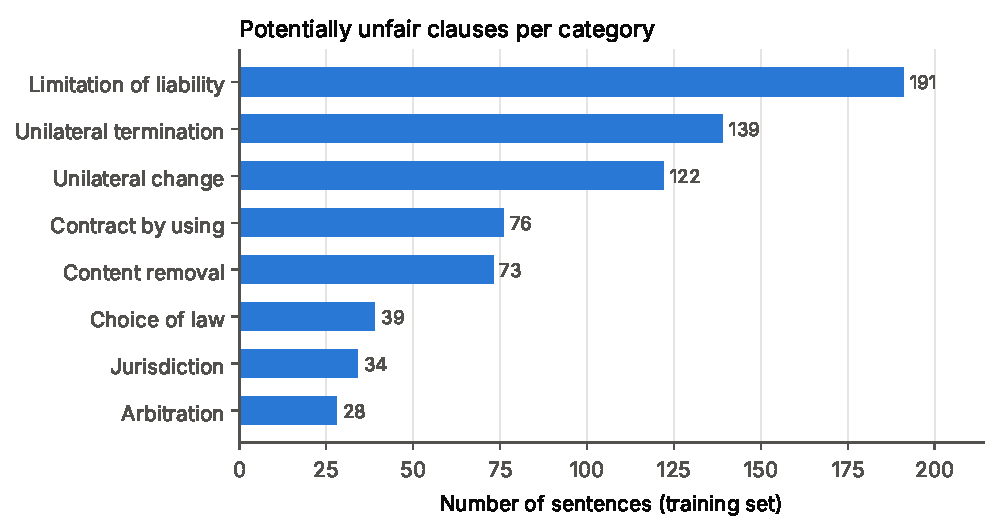
\includegraphics[width=0.62\textwidth]{label_distribution.pdf}
\caption{Potentially unfair sentences per category in the UNFAIR-ToS training set.}
\label{fig:labels}
\end{figure}

\subsection{Multilingual Claudette corpus}
\label{sec:data-multi}

For the fairness extension we use the corpus of Drawzeski et al.~\citep{drawzeski2021}: 25 Terms of Service, each in English, German, Italian and Polish (25,929 sentences, versions of about 2021, licence CC BY-NC 2.5). Every sentence has an unfairness level (clearly fair, potentially unfair, clearly unfair) and category tags. We map potentially and clearly unfair sentences to ``unfair'', and the tags to the eight UNFAIR-ToS categories. The annotation is consistent across languages: 9.3--9.9\% of the sentences are unfair in every language.

Many of these contracts are later versions of contracts in UNFAIR-ToS: 42.1\% of the English sentences are near-duplicates of UNFAIR-ToS sentences, and therefore also of our knowledge base. To measure performance on unseen contracts, the evaluation set keeps only the 10 companies whose English version overlaps with UNFAIR-ToS for less than 10\% of its sentences: Electronic Arts, Facebook, Garmin, Grindr, Mozilla, Pinterest, Quora, Ryanair, Weebly and Yelp. It also removes the remaining English near-duplicates and the sentences tagged only with the privacy category, which UNFAIR-ToS does not have. Table~\ref{tab:multi} gives the result. The sentences of the four versions of a contract are not aligned one to one, so languages are compared as groups, not sentence by sentence.

\begin{table}[ht]
\centering\small
\caption{Multilingual evaluation set (10 companies).}
\label{tab:multi}
\begin{tabular}{@{}lrrrr@{}}
\toprule
& English & German & Italian & Polish \\
\midrule
Sentences & 2,366 & 2,270 & 2,473 & 2,714 \\
Potentially unfair & 219 & 219 & 229 & 238 \\
\bottomrule
\end{tabular}
\end{table}

\section{Legal knowledge base}
\label{sec:kb}

The knowledge base (\texttt{knowledge\_base/}, YAML files written by us) contains the legal knowledge the RAG system retrieves. It has four kinds of documents, 5,584 in total.
\begin{itemize}
  \item \textbf{Legal provisions (20).} Articles 3(1), 3(2), 3(3), 4(1), 5 and 6(1) of Directive 93/13, ten points of its Annex, Articles 17--19 of the Brussels~Ia Regulation, Article 6(2) of Rome~I, and two CJEU judgments: \emph{Oc\'eano}~\citep{cjeu_oceano} and \emph{VKI v Amazon}~\citep{cjeu_amazon}. Each provision is summarised in our own words, with its exact reference and a link to the official text, so every statement can be checked.
  \item \textbf{Category cards (8).} For each category: a definition, the Claudette criteria for clearly fair, potentially unfair and clearly unfair clauses~\citep{lippi2019claudette}, why the clause matters for consumers, and its legal basis. The cards are part of the system prompt of every LLM-based system.
  \item \textbf{Legal rationales (89).} Specific practices that make a clause unfair or fair, for example ``the provider may terminate the account for any reason, without notice''. 78 are paraphrased from the rationales of Ruggeri et al.~\citep{ruggeri2022memory} for arbitration, unilateral change, content removal, termination and limitation of liability. We wrote the other 11, for the remaining three categories and for clearly fair practices. 74 rationales describe potentially unfair practices, 11 clearly unfair ones and 4 clearly fair ones. Each rationale links to the provisions it relies on.
  \item \textbf{Examples (5,467).} The UNFAIR-ToS training sentences with their expert labels (626 unfair, 4,841 fair). The 65 training sentences that also occur in the validation or test set are removed.
\end{itemize}

Every document has an id that the language model must cite, which is what makes the explanations checkable. A validator, covered by unit tests, checks that ids are unique, that categories match the dataset labels and that every reference points to an existing provision or source. Figure~\ref{fig:kb-example} shows a rationale and a provision as the model sees them.

\begin{figure}[ht]
\centering\small
\fbox{\begin{minipage}{0.94\textwidth}\raggedright
\texttt{[ter.any\_reasons]} Unilateral termination -- clearly unfair: The provider may terminate or suspend for any reason, without cause, or for reasons it does not specify.\\[3pt]
\texttt{[dir93.annex.1q]} Directive 93/13/EEC, Annex, point 1(q) -- Hindering legal action: Terms that exclude or hinder the consumer's right to take legal action or use other remedies, in particular by requiring disputes to go exclusively to arbitration not covered by legal provisions [\ldots]\\[3pt]
\texttt{[ex.train-2548]} (unfair: ch, ter) ``we reserve the right to modify or terminate the service or your access to the service for any reason, without notice, at any time, and without liability to you .''
\end{minipage}}
\caption{A rationale, a provision and an example of the knowledge base, as they appear in a prompt.}
\label{fig:kb-example}
\end{figure}
